
\chapter{Reducing Binary PR to Formula Satisfiability}\label{chap:bpr_fsat}
In this chapter, we finally encode \PR{} over a binary alphabet as a Boolean formula. This formula will not be in CNF, yet.
The main idea of the encoding is to explicitly unfold the tableau induced by the \BPR{} instance.
As we are working over a binary alphabet, each character of the involved strings can be accomodated by one Boolean variable. A satisfying assignment to the formula will therefore resemble a sequence of valid rewrites, starting with the initial string and ending up with a string satisfying the final substring constraint.
The formula $\phi$ we generate is a conjunction of three gadgets: a formula $\phi_{\textsf{init}}$ enforcing that the first line of the tableau matches the initial string, a formula $\phi_{\textsf{trans}}$ encoding that the individual lines follow from each other according to the rewrite windows, and a formula $\phi_{\textsf{final}}$ which makes the final substring constraint hold. 

\newcommand{\formula}{\mathcal{F}}
\setCoqFilename{Undecidability.L.Complexity.Problems.FSAT}
\section{Formula Satisfiability (FSAT)}
We start by introducing a generalised variant of \SAT{} that does not require the formula to be in CNF.

Formulas are defined inductively: 
\mnote[formula]{$\formula$}
\[f : \formula \defeq \btrue \bnfmid v \bnfmid f_1 \lor f_2 \bnfmid f_1 \land f_2 \bnfmid \lnot f \qquad (v : \bvar) \]

One can directly derive the operators $\land$ and $\lor$ for more than two operands, which we will denote by $\bigwedge_{f \in l} f$ and $\bigvee_{f \in l} f$ for $ l : \listsof{\formula}$. 

Assignments $a : \assgn$ are defined in the same way as for CNFs, see Section~\ref{sec:sat}.
An \coqlink[evalFormula]{evaluation function} $\eval : \assgn \rightarrow \formula \rightarrow \bool$ can be derived in the canonical way. We say that an assignment $a$ \coqlink[satisfies]{satisfies} $f$, written $a \models f$, if $\evalA{a}{f} = \btrue$.

\begin{definition}[Formula Satisfiability][FSAT]
  \mnote[FSAT]{\fsat{}}
  $\fsat{}~f \defeq \exists a, a \models f$
\end{definition}

We could prove that \fsat{} is in \NP{} using the same notion of small assignments as for CNF satisfiability. This will, however, already follow from the reduction of \fsat{} to \SAT{} in Chapter~\ref{chap:fsat_sat}. 

\paragraph{Explicit Assignments}
The assignments we use, where we just store a list of variables to which the value $\btrue$ is assigned and to all other variables the value $\bfalse$ is assigned implicitly, are quite indirect and unstructured. 
For the rest of this chapter a more explicit characterisation bearing resemblance to the Boolean strings used by \BPR{} will be quite convenient.
One possible characterisation is a list of Booleans $e : \listsof{\bool}$ together with a start index $s$, where the value $e[i]$ at position $i$ of this list is the value assigned to variable $s + i$. To variables outside the range $[s, s+\length{e})$, the value $\bfalse$ is assigned.

As we will be working with ranges of variables $[\textsf{start}, \textsf{start} + \textsf{len})$ a lot throughout this chapter, we introduce the notation \mnotec{$[s .. +l)$} instead of $[s, s+l)$, which makes the notation less redundant. In the following, we use the letter $I$ to denote variable ranges of this form.

We can naturally convert back and forth between such explicit assignments and assignments $a : \assgn$.
First, we present a function that generates an explicit assignments for the variables in range $[\text{start}, \text{start} + \text{len})$. 
\setCoqFilename{Undecidability.L.Complexity.Reductions.Cook.BinaryPR_to_FSAT}%
\newcommand{\explicitA}{\textsf{explicitAssgn}}
\begin{align*}
  \mnote[explicitAssignment]{explicitA}\explicitA &: \assgn \rightarrow \nat \rightarrow \nat \rightarrow \listsof{\nat} \\
  \explicitA~a~\textsf{start}~0 &\defeq \nil \\
  \explicitA~a~\textsf{start}~(\natS{\textsf{len}}) &\defeq \explicitA~a~\textsf{start}~\textsf{len} \concat [(\textsf{start} + \textsf{len}) \oset{?}{\in}{+1.2} a]
\end{align*}
We use the notation $a[s ..+l) \defeq \explicitA~a~s~l$ and may also write \mnotec{$a[I]$} for a variable range $I$.
\begin{lemma}[Properties of \explicitA]\leavevmode
  \begin{enumerate}
    \coqitem[explicitAssignment_length] $\length{\explicitA~a~\textsf{start}~\textsf{len}} = \textsf{len}$
    \coqitem[explicitAssignment_nth] $k < \textsf{len} \rightarrow (\explicitA~a~\textsf{start}~\textsf{len})[k] = \OSome{(\evalA{a}{(\textsf{start} + k)})}$
    \coqitem[explicitAssignment_app] $\explicitA~a~s~(l_1 + l_2) = \explicitA~a~s~l_1 \concat \explicitA~a~(s + l_1)~l_2$ 
  \end{enumerate}
\end{lemma}

%\newcommand{\expandA}{\textsf{expandAssgn}}
%Of course, we can go back to a full assignment: 
%\begin{proposition}[][expAssgn_to_assgn] 
  %Let $e : \listsof{\bool}$ and a start variable index $s$ be given. Then:
  %\[\sigtype{a}. \forall x, x \in a \leftrightarrow x \ge s \land e[x-s] = \OSome{\btrue} \]
  %\coqlink[expAssgn_to_assgn_inv]{Moreover}, if $a$ satisfies $\forall x, x \in a \leftrightarrow x \ge s \land e[x-s] = \OSome{\btrue}$, then:
  %\[\explicitA~a~s~(\length{e}) = e \]
%\end{proposition}

\newcommand{\projVars}{\textsf{projVars}}
Given an explicit assignment $e$, we can project out the assignment to a particular range of variables $I = [\textsf{start}.. +\textsf{len})$:
\mnote[projVars]{$e[I]$}
\[e[I] = e[\textsf{start}..+\textsf{len}) \defeq (e[\textsf{len} ..])[.. \textsf{start}).\] 
The subscripting notation thus is overloaded for full assignments and for explicit assignments, but this will not pose a problem as it will always be clear from the context what we mean.

\section{Encoding Properties using Boolean Formulas}
Based on explicit assignments, we now present ways to encode predicates using formulas $f : \formula$ and show that this representation is closed under conjunction and disjunction, the main composition operations we need for the reduction.

\newcommand{\encodesPred}{\textsf{encodesPredAt}}
\begin{definition}[Encoding of Predicates][encodesPredicateAt]
  \mnote[encodesPredicateAt]{\encodesPred}
  A formula $f$ encodes a predicate $p : \listsof{\bool} \rightarrow \Prop$ on a range of variables $I = [\textsf{start}.. + \textsf{len})$ if, for every assignment $a$, $a \models f$ is equivalent to satisfaction of $p$ under the partial assignment given by $I$:
  \[\encodesPred~\textsf{start}~l~f~p \defeq \forall a, a \models f \leftrightarrow p~(a[\textsf{start}.. + l]) \]
\end{definition}

This encoding scheme is rather simple: we can only prove statements about contiguous ranges of variables. 
An elaborate definition allowing a more fine-grained control would be possible, but over-complicated for our simple use case.

To stay in line with the variable range notation, we also write $\encodesPred~I~f~p$ for a range of variables $I$.

A rather trivial but important fact is that \encodesPred{} is extensional with respect to the encoded predicate. This will be quite convenient for proving correctness of encodings by switching to an equivalent characterisation of the predicate we want to encode.
\begin{fact}[Extensionality][encodesPredicateAt_extensional]\label{fact:enc_congruent}
  Let $\forall e, \length{e} = l \rightarrow p_1~e \leftrightarrow p_2~e$. Then
  \[\encodesPred~s~l~f~p_1 \leftrightarrow \encodesPred~s~l~f~p_2.\]
\end{fact}

\newcommand{\encodeLiteral}{\textsf{encodeLiteral}}
As a first example, we define the encoding of a literal: 
\[\encodeLiteral~v~\textsf{sign} : \formula \defeq \ITE{\textsf{sign}}{v}{\lnot v} \mnote[encodeLiteral]{\encodeLiteral}\]
As one would expect, the formula $\encodeLiteral~v~s$ forces variable $v$ to take the value s: 
\begin{proposition}[Correctness of \encodeLiteral][encodeLiteral_correct]
  \[\encodesPred~v~1~(\encodeLiteral~v~s) (\lambda l. l = [s])\]
\end{proposition}

Next, we show that conjunction and disjunction of formulas correspond to conjunction and disjunction of represented predicates. One problem with this is that the two predicates may talk about different variable ranges $I_1$ and $I_2$. 
Our simple representation model does not allow to accurately depict this, hence the new predicate will talk about the smallest range of variables $I$ that contains $I_1$ and $I_2$. We write this as $I = I_1 \sqcup I_2$.
\newcommand{\cStart}{\textsf{combStart}}
\newcommand{\cLength}{\textsf{combLength}}
\begin{align*}
  \cStart~s_1~s_2 &\defeq \min~s_1~s_2 \mnote[combinedStart]{\cStart}\\
  \cLength~s_1~s_2~l_1~l_2 &\defeq \max~(s_1 + l_1) (s_2 + l_2) - \min~s_1~s_2 \mnote[combinedLength]{\cLength}\\
  [s_1.. + l_1) \sqcup [s_2.. + l_2) &\defeq [\cStart~s_1~s_2.. +\cLength~s_1~s_2~l_1~l_2) \mnote{$I_1 \sqcup I_2$}
\end{align*}

Using $e[s..+l]$, we can restore the assignments to $I_1$ and $I_2$ given an assignment to $I_1 \sqcup I_2$:
\begin{proposition}\label{prop:comb_proj}
  Let $I_1 = [s_1 ..+ l_1)$ and $I_2 = [s_2 ..+l_2)$. 
  \begin{enumerate}
    \coqitem[projVars_combined1] $a[I_1] = (a[I_1 \sqcup I_2])[(s_1 - \cStart~s_1~s_2) .. + l_1]$
    \coqitem[projVars_combined2] $a[I_2] = (a[I_1 \sqcup I_2])[(s_2 - \cStart~s_1~s_2) .. + l_2]$
  \end{enumerate}
\end{proposition}

Now, we have all the tools necessary to combine the encoding of two predicates:
\begin{lemma}[Encoding of $\land$ and $\lor$]
  Let $I_1 = [s_1 .. + l_2)$ and $I_2 = [s_2 .. + l_2)$.
  Assume that $\encodesPred~s_1~l_1~f_1~p_1$ and $\encodesPred~s_2~l_2~f_2~p_2$. 
  \begin{enumerate}
    \coqitem[encodesPredicate_and]
      $\begin{aligned}[t]
        &\encodesPred ~(I_1 \sqcup I_2) (f_1 \land f_2) \\ 
        &\quad (\lambda e. p_1 (e[s_1 - \cStart~s_1~s_2 .. +l_1]) \land p_2 (e[s_2 - \cStart~s_1~s_2 .. + l_2]))
      \end{aligned}$
   \coqitem[encodesPredicate_or]
      $\begin{aligned}[t]
        &\encodesPred ~(I_1 \sqcup I_2) (f_1 \lor f_2) \\ 
        &\quad (\lambda e. p_1 (e[s_1 - \cStart~s_1~s_2 .. +l_1]) \lor p_2 (e[s_2 - \cStart~s_1~s_2 .. + l_2]))
      \end{aligned}$
  \end{enumerate}
\end{lemma}
\begin{proof}
  Straightforward using Proposition~\ref{prop:comb_proj}.
\end{proof}

By conjoining formulas encoding single literals, a list $L : \listsof{\bool}$ can be encoded by forcing a range of variables to be equal to the list. 
\newcommand{\encodeList}{\textsf{encodeList}}%
\begin{align*}
  \mnote[encodeListAt]{\encodeList}
  \encodeList~s~\nil &\defeq \btrue \\
  \encodeList~s~(l :: L) &\defeq \encodeLiteral~s~l \land \encodeList~(\natS{s})~L
\end{align*}

\begin{proposition}[Correctness of \encodeList][encodeListAt_encodesPredicate]
  \[\encodesPred~s~(\length{L})~(\encodeList~s~L)~(\lambda e. L = e)\]
\end{proposition}

\encodeList{} will be the basic ingredient of encoding \PR{}. 

\section{Reduction to \fsat{}}
In this section, we show how to encode the three subformulas $\phi_{\textsf{init}}, \phi_{\textsf{trans}}, \phi_{\textsf{final}}$. 
As most of the encodings are straightforward to see from the definition of \PR{}, we only give an informal description for some of them. 

From now on, fix a \BPR{} instance $(o, \omega, x_0, R, \Rfinal, t)$ that satisfies the syntactic constraints of Definition~\ref{def:pr}.
For our convenience, we define $m \defeq \length{x_0}$ to be the length of each of the tableau's lines. \mnote[llength]{$m$}

The variable layout of the formula we produce is demonstrated by Figure~\ref{fig:varlayout}
\begin{figure}
  \begin{center}
    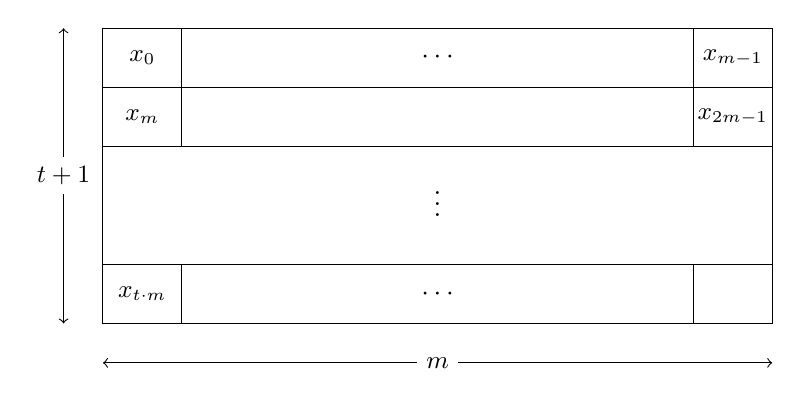
\begin{tikzpicture}
      \draw (1.5, -0.75) -- (1.5, 3) -- (10, 3) -- (10, -0.75) -- (1.5, -0.75);
      %\draw (2, -4) -- (2, 3);
      %\draw (2.5, 3) -- (1.5, 2);
      %\draw (9.5, -4) -- (9.5, 3);
      \draw (1.5, 2.25) -- (10, 2.25);
      \draw (1.5, 0) -- (10, 0);
      \draw (1.5, 1.5) -- (10, 1.5);

      \draw (2.5, 1.5) -- (2.5, 3);
      \draw (9, 1.5) -- (9, 3);
      \draw (2.5, 0) -- (2.5, -0.75);
      \draw (9, 0) -- (9, -0.75);
      
      \node at (2, 2.625) {\small$x_0$};
      \node at (9.5, 2.625) {\small$x_{m-1}$};
      \node at (2, 1.875) {\small$x_m$};
      \node at (9.5, 1.875) {\small$x_{2m-1}$};
      \node at (2, -0.375) {\small$x_{t\cdot m}$};
      %\node at (9.75, 0.25) {\small$x_{(t+1) \cdot m -1}$};

      %\draw (4.5, 3) -- (4.5, 2);
      %\draw (5, 3) -- (5, 2);
      %\draw (5.5, 3) -- (5.5, 2);
      %\draw (6, 3) -- (6, 2);
      %\draw (7, 3) -- (7, 2);
      %\draw (7.5, 3) -- (7.5, 2);
      %\draw (8, 3) -- (8, 2);
      %\draw (9, 3) -- (9, 2);

      %\node at (2.25, 2.75) {\textvisiblespace};
      %\node at (3.5, 2.75) {$\ldots$};
      %\node at (4.75, 2.75) {\textvisiblespace};
      %\node at (5.25, 2.75) {\small $q_0^{\blank}$};
      %\node at (5.75, 2.75) {\small $\sigma_1$};
      %\node at (6.5, 2.75) {$\ldots$};
      %\node at (7.25, 2.75) {\small $\sigma_l$};
      %\node at (7.75, 2.75) {\textvisiblespace};
      %\node at (8.5, 2.75) {$\ldots$};
      %\node at (9.25, 2.75) {\textvisiblespace};

      \node at (5.75, -0.375) {$\cdots$};
      \node at (5.75, 2.625) {$\cdots$};
      \node at (5.75, 0.875) {$\vdots$};
      %\node at (9.75, -0.375) {$\vdots$};

      \path[<->] (1, -0.75) edge node[fill=white, anchor=center, pos= 0.5] {\small $t+1$} (1, 3);
      \path[<->] (1.5, -1.25) edge node[fill=white, anchor=center, pos=0.5] {\small $m$} (10, -1.25);
    \end{tikzpicture}     
  \end{center}
  \caption{The variable layout of the constructed \fsat{} instance does directly mirror the layout of the \PR{} strings in a tableau.}\label{fig:varlayout}
\end{figure} 

We start with the encoding of $\phi_{\textsf{trans}}$. This is most intuitive when looking at the explicit characterisation of validity (see Definition~\ref{def:valid_exp}): we have a big conjunction over all pairs of subsequent lines for which we have to enforce validity. Validity can be encoded as a conjunction over the offsets at which a window needs to hold, and at each position we have a disjunction over all possible rewrite windows. 
First of all, we need to be able to encode a single rewrite window. As a rewrite windows just encodes two lists, this is straightforward to derive as a conjunction for premise and conclusion. Since the premise of the window needs to match in one line of the tableau while the conclusion needs to hold for the next line, the encoding is parameterised over two indices $s_1$ and $s_2$ giving the respective start of the encoding. 
\newcommand{\encodeWindow}{\textsf{encodeWindow}}
\[ \encodeWindow~s_1~s_2~w \defeq \encodeList~s_1~(\prem~w) \land \encodeList~s_2~(\conc~w)\mnote[encodeWindowAt]{\encodeWindow} \]
The correctness statement of course also needs to range over all the variables between the two starting indices.
\begin{proposition}[Correctness of \encodeWindow][encodeWindowAt_encodesPredicate]
  Let $s, l : \nat$ and $win : \win{\bool}$.
  \begin{align*}
    \encodesPred~s~(l + \omega)~&(\encodeWindow~s~(s + l)~win)\\
    & (\lambda e. e[0 ..+\omega) = \prem~win \land e[l ..+\omega) = \conc~win )
  \end{align*}
\end{proposition}

\newcommand{\encodeWindows}{\textsf{encodeWindows}}
This can be lifted to express that one of the windows of $R$ holds at a given position by computing a disjunction over the list of windows. 
We assume a function $\encodeWindows : \nat \rightarrow \nat \rightarrow \formula$ \mnote[encodeWindowsAt]{\encodeWindows} taking the two start indices for that purpose, without going into more detail.
\begin{proposition}[Correctness of \encodeWindows][encodeWindowsAt_encodesPredicate]
  Let $s, l : \nat$.
  \begin{align*}
    \encodesPred~s~(l + \omega)~&(\encodeWindows~s~(s + l)) \\
                                &(\lambda e. \exists w, w \in R \land e[0 ..+ \omega) = \prem~w \land e[l .. + \omega) = \conc~w) 
  \end{align*}
\end{proposition}

A bit more interesting is the function needed to encode all windows at every offset of a string. Technically, this is a conjunction over all possible offsets. The fact that the windows only need to hold at multiples of $o$ is a minor inconvenience as this means that we cannot define the function computing the formula using direct structural recursion over the position at which we encode the windows next\footnote{Coq requires functions to be structurally recursive.}.
Instead, we employ a step index which is initialised to the length $m = \length{x_0}$ of the lines of the tableau to make the function structurally recursive.
\newcommand{\encodeWindowsLine}{\textsf{encodeWindowsLine}}
\begin{align*}
  &\encodeWindowsLine'~\textsf{step}~l~s_1~s_2 \defeq \textbf{if}~{l \oset{?}{<}{+0.9} \omega}~\textbf{then}~{\btrue} \mnote[encodeWindowsLine]{\encodeWindowsLine}\\
  &\quad\textbf{else}~\match \textsf{step} \withl 
    0 \Rightarrow \btrue \withm \natS{\textsf{step}}  
    \begin{aligned}[t]
      \Rightarrow&~\encodeWindows~s_1~s_2  \\
      \land &~\encodeWindowsLine'~\textsf{step}~(l - o)~(s_1 + o)~(s_2 + o)\withr
    \end{aligned} \\[0.7em]
            &\encodeWindowsLine~\textsf{step}~s \defeq \encodeWindowsLine'~m~m~s~(s + m) 
\end{align*}
Intuitively, the parameter $s_1$ of $\encodeWindowsLine'$ determines the first index starting at which the premises of the windows are placed, while $s_2$ is the starting index of the conclusions.

\todo{find solution for encodeWindowsLine box}
\begin{proposition}[Correctness of $\encodeWindowsLine$][encodeWindowsInLineP_encodesPredicate]
  Let $l \le m$. 
  \begin{align*}
    \encodesPred~s~(l + m)~&(\encodeWindowsLine'~l~l~s~(s + m)) \\
                                      &(\lambda e. (e[0 ..+l)) \strent{R} (e[m .. +l))
  \end{align*} 
  \coqlink[encodeWindowsInLine_encodesPredicate]{Moreover}, we have
  \[\encodesPred~s~(2 \cdot m) (\encodeWindowsLine~s) (\lambda e. (e[0 ..+m)) \strent{R} (e[m ..+m)) \]
\end{proposition}
\begin{proof}
  The second statement is the first one instantiated with $l \defeq \length{x_0}$. 
  For the first statement, we use strong induction on $l$.
\end{proof}

Now we can obtain the formula \mnotec[encodeWindowsInAllLines]{$\phi_{\textsf{trans}}$} by forming a conjunction over all lines of the tableau.
\begin{lemma}[Correctness of $\phi_{\textsf{trans}}$][encodeWindowsInAllLines_encodesPredicate]
  \begin{align*}
    \encodesPred~&0~((\natS{t}) \cdot m)~\phi_{\textsf{trans}} \\
                                                   &(\lambda e. \forall 0 \le i < t, ((e[i \cdot m..+m)) \strent{R} (e[(\natS{i}) \cdot m ..+m)))
  \end{align*}
\end{lemma}

The final constraint can be encoded similarly: we have a nested disjunction over the strings in $\Rfinal$ and the possible positions at which they can match. For the latter, remember that the final substrings need to match at positions which are multiples of the offset $o$. Therefore, we employ a step-indexing technique similar to the one for \encodeWindowsLine. 

\begin{lemma}[Correctness of $\phi_{\textsf{final}}$][encodeFinalConstraint_encodesPredicate]
  \mnote[encodeFinalConstraint]{$\phi_{\textsf{final}}$}
  \[\encodesPred~(t \cdot m)~m~\phi_{\textsf{final}}~(\lambda e. e \models \Rfinal) \]
\end{lemma}

Finally, the initial constraint is simply an instance of \encodeList: the first $\length{x_0}$ variables have to match $x_0$. 
Therefore, in the end the whole formula is
\[ \phi \defeq \encodeList~0~x_0 \land \phi_{\textsf{trans}} \land \phi_{\textsf{final}}.\mnote[encodeTableau]{$\phi$} \]

\begin{lemma}[Correctness of $\phi$][encodeTableau_encodesPredicate]\label{lem:phi_correct}
  \begin{align*}
    \encodesPred~&0~((\natS{t}) \cdot m)~\phi \\
                 &(\lambda e. \begin{aligned}[t]
                  &e[0.. + m) = x_0 \\
                   \land &  (\forall 0 \le i < t, ((e[i \cdot m..+m)) \strent{R} (e[(\natS{i}) \cdot m..+m))) \\
                   \land & e[t \cdot m .. + m) \models \Rfinal)
                \end{aligned}
  \end{align*}
\end{lemma}

\begin{theorem}[\BPR{} Reduces to \fsat{}][BinaryPR_to_FSAT]
  \[\fsat~\phi \leftrightarrow \exists x_t, x_0 \strent{R}^t x_t \land x_t \models \Rfinal \]
\end{theorem}
\begin{proof}\leavevmode
  \begin{description}
    \item[$\rightarrow$:]
      As $\fsat{}~\phi$ holds, we have a satisfying assignment $a$. 
      By Lemma~\ref{lem:phi_correct}, the corresponding explicit assignment to the first $(\natS{t}) \cdot \length{x_0}$ variables witnesses a valid rewrite sequence satisfying the final constraint. 
      We prove that $e[0 ..m) \strent{R}^t e[t \cdot m ..+ m)$ by switching to $\prescript{t}{}{\strent{R}}$ and doing an induction on $t$.
    \item[$\leftarrow$:]
      From the proof that the initial string rewrites in $t$ steps to a final string we have to generate a sequence of intermediate strings that together form a satisfying assignment. 
      For this, we generalise to arbitrary strings $x, y$ with $\length{x} = \length{x_0} = m$ and show that, if $x \strent{R}^n y$, then there exists $e$ with $\length{e} = (\natS{n}) \cdot m$ and 
      \begin{align*}
        &e[0..+ m) = x \land e[n \cdot m ..+ m) = y \\
        \land & (\forall 0 \le i < n, (e[i \cdot m ..+ m)) \strent{R} e[(\natS{i}) \cdot m ..+ m))).
      \end{align*}
      This statement follows by an induction on $x \strent{R} y$.
  \end{description}
\end{proof}

\section{Mechanisation}
We again comment on some aspects of the mechanisation.

As in the previous chapter, we have to treat non-wellformed instances separately by first deciding wellformedness and mapping violating instances to a trivial no-instance. 

A major inconvenience is that many of the representation proofs are somewhat repetitive and mainly rely on inductively forming conjunctions and disjunctions of formulas. Except for the two functions which need step-indexing, these can be taken care of by a few lemmas that allow to form the disjunction or conjunction of a list of formulas at a fixed position or by replicating a formula parameterised by the index of the first variable it uses at various positions for a given offset between the replications. 
The authors of~\cite{Larchey-WendlingForster:2019:H10_in_Coq} face a similar problem in encoding certain predicates using Diophantine equations. They come up with Coq tactics that can largely automate the process of finding an encoding and proving its correctness if the predicate has a shape that is already known, using the Coq unification mechanism. If the predicate is not in a known shape, extensionality can be used to bring it into an equivalent shape, similar to our Fact~\ref{fact:enc_congruent}.
The key idea of their approach is to use Sigma types that informatively bundle the encoding and its proof of correctness. 
Sadly, a similar trick can not be applied in our setting: Sigma types (or even their computational part) currently are not extractable to L. Thus, it seems unavoidable to explicitly define the formula encoding a particular predicate.

As both \BPR{} and \fsat{} are directly extractable, we need not define separate flat versions. Thus, we obtain the following polynomial-time reduction:
\begin{theorem}[][BinaryPR_to_FSAT_poly]
  $\BPR{} \redP{} \fsat{}$
\end{theorem}
